% Master's thesis poster -- A1 portrait, dark theme, two columns. Compile with xelatex here.
\documentclass[final]{article}

\usepackage[paperwidth=594mm,paperheight=841mm,top=15mm,bottom=13mm,left=14mm,right=14mm]{geometry}
\usepackage{fontspec}
\usepackage{graphicx}
\usepackage[table]{xcolor}
\usepackage[most]{tcolorbox}
\usepackage{tabularx}
\usepackage{ragged2e}
\usepackage{amsmath}
\usepackage{amssymb}
\usepackage{fontawesome5}
\usepackage{anyfontsize}
\usepackage{hyperref}

\graphicspath{{../assets/}{../../output/figures/03_build/}{../../output/figures/04_descriptive/}{.}}

\setmainfont{Helvetica Neue}
\setsansfont{Helvetica Neue}
\renewcommand{\familydefault}{\sfdefault}

\definecolor{bg}{HTML}{25313A}
\definecolor{panel}{HTML}{2E3C46}
\definecolor{darkcell}{HTML}{212C34}
\definecolor{ink}{HTML}{DBE0E4}
\definecolor{white}{HTML}{FFFFFF}
\definecolor{amber}{HTML}{F2A65A}
\definecolor{amberlt}{HTML}{FFC489}
\definecolor{sky}{HTML}{8ABAE0}
\definecolor{muted}{HTML}{96A4AE}
\definecolor{rule}{HTML}{415159}

\pagecolor{bg}\color{ink}\pagestyle{empty}\setlength{\parindent}{0pt}

\newlength{\colheight}\setlength{\colheight}{681mm}
\newcommand{\col}{0.485\textwidth}
\newcommand{\gp}{\vspace{9mm}}           % fixed top-driven gap between elements
\newcommand{\sechead}[2]{{\color{amber}\bfseries #1}\hspace{3.5mm}#2}

\newtcolorbox{panel}[1]{
  enhanced, colback=panel, colframe=panel, boxrule=0pt, arc=3mm,
  left=8.5mm, right=8.5mm, top=5.8mm, bottom=6.8mm,
  coltitle=white, colbacktitle=panel,
  fonttitle=\bfseries\fontsize{31pt}{36pt}\selectfont,
  title={#1}, toptitle=1.4mm, bottomtitle=4mm,
  fontupper=\fontsize{24pt}{33pt}\selectfont\color{ink}\justifying\setlength{\parindent}{0pt},
}
\newtcolorbox{conclbox}[1]{
  enhanced, colback=panel, colframe=amber, boxrule=1.8pt, arc=3mm,
  left=8.5mm, right=8.5mm, top=5.8mm, bottom=7mm,
  coltitle=amber, colbacktitle=panel,
  fonttitle=\bfseries\fontsize{31pt}{36pt}\selectfont,
  title={#1}, toptitle=1.4mm, bottomtitle=4mm,
  fontupper=\fontsize{24pt}{34pt}\selectfont\color{white}\justifying\setlength{\parindent}{0pt},
}

\newcommand{\figtitle}[1]{{\bfseries\color{amber}\fontsize{23pt}{27pt}\selectfont #1\par}\vspace{2.4mm}}
\newcommand{\figcap}[1]{\vspace{1.8mm}{\itshape\color{muted}\fontsize{17pt}{21pt}\selectfont #1\par}}
\newtcolorbox{whitecard}{colback=white, colframe=white, boxrule=0pt, arc=2mm,
  left=1.6mm, right=1.6mm, top=1.6mm, bottom=1.6mm, halign=center}

% ============================================================================
\begin{document}

% ---- Title band -------------------------------------------------------------
\noindent
\begin{minipage}[c]{0.80\textwidth}
  {\bfseries\color{white}\fontsize{56pt}{62pt}\selectfont When Rough Seas Become Deadlier\par}
  \vspace{5.5mm}
  {\color{sky}\fontsize{31pt}{37pt}\selectfont
   Migrant mortality and the 2017 Italy--Libya Memorandum on the Central Mediterranean Route\par}
  \vspace{6.5mm}
  {\color{muted}\fontsize{22pt}{26pt}\selectfont
   \textbf{\color{ink}Giorgio Coppola -- MSc of Data Science for Public Policy}, Hertie School
   \;\textbar\; \color{ink}Supervisor: \textbf{Prof.\ Dr.\ Asya Magazinnik}\par}
\end{minipage}\hfill
\begin{minipage}[c]{0.17\textwidth}
  \raggedleft
  \begin{tcolorbox}[colback=white,colframe=white,boxrule=0pt,arc=2mm,
                    left=3mm,right=3mm,top=3mm,bottom=3mm,width=70mm,height=32mm,
                    valign=center,nobeforeafter]
    
\includegraphics[width=62mm]{hertie-school-logo.png}
  \end{tcolorbox}
\end{minipage}

\vspace{7mm}
{\color{amber}\rule{\textwidth}{2.2pt}}
\vspace{8mm}

% ---- Two columns (top-aligned, uniform gaps) --------------------------------
\noindent
% ===== LEFT COLUMN ==========================================================
\begin{minipage}[t]{\col}
  \vspace{0pt}
  \begin{panel}{\sechead{1}{Motivation: risk at sea}}
    The Central Mediterranean route (\textbf{CMR}) is the world's deadliest migration route:
    \textbf{\color{white}20,368} recorded deaths in the 2014--2023 corridor sample alone.
    In 2017 the Italy--Libya Memorandum (\textbf{MoU}) turned EU policy from rescue toward
    interception, financing the Libyan Coast Guard and constraining NGO search-and-rescue
    (\textbf{SAR}). Crossings fell, but whether each crossing became \emph{safer}, or merely
    less rescued, stayed open. The key margin is therefore \textbf{risk per crossing}.
  \end{panel}
  \gp

  \begin{panel}{\sechead{2}{Mechanism: SAR and risk moderation}}
    Sea state acts through two channels. Rough seas \textbf{deter departures}, lowering
    recorded deaths; but conditional on departing, they raise the chance of distress,
    capsize and death. \textbf{SAR moderates this second, per-crossing channel}. As
    European state-led and NGO-led SAR withdrew from 2017 onward, that buffer should weaken, so the same
    seas should map into \textbf{more} recorded deaths. The prediction is a positive
    post-MoU shift in the weather--mortality slope.
  \end{panel}
  \gp

  \begin{panel}{\sechead{3}{Data: daily route-level time series}}
    A daily time series for the corridor, \textbf{January 2014--May 2023}, combining ERA5 wave
    height (\textbf{SWH}), \textbf{UNITED} and \textbf{IOM} recorded deaths, Frontex
    interceptions, and Libyan and Tunisian coast-guard pull-backs. The main regressor is
    the lagged five-day mean of wave height; the regime split is dated to the MoU signing
    on \textbf{2 February 2017}. This links sea state, mortality and crossing proxies on a
    common daily calendar.
  \end{panel}
  \gp

  \figtitle{Fig 1 \textbar\ From rescue to interception}
  \begin{whitecard}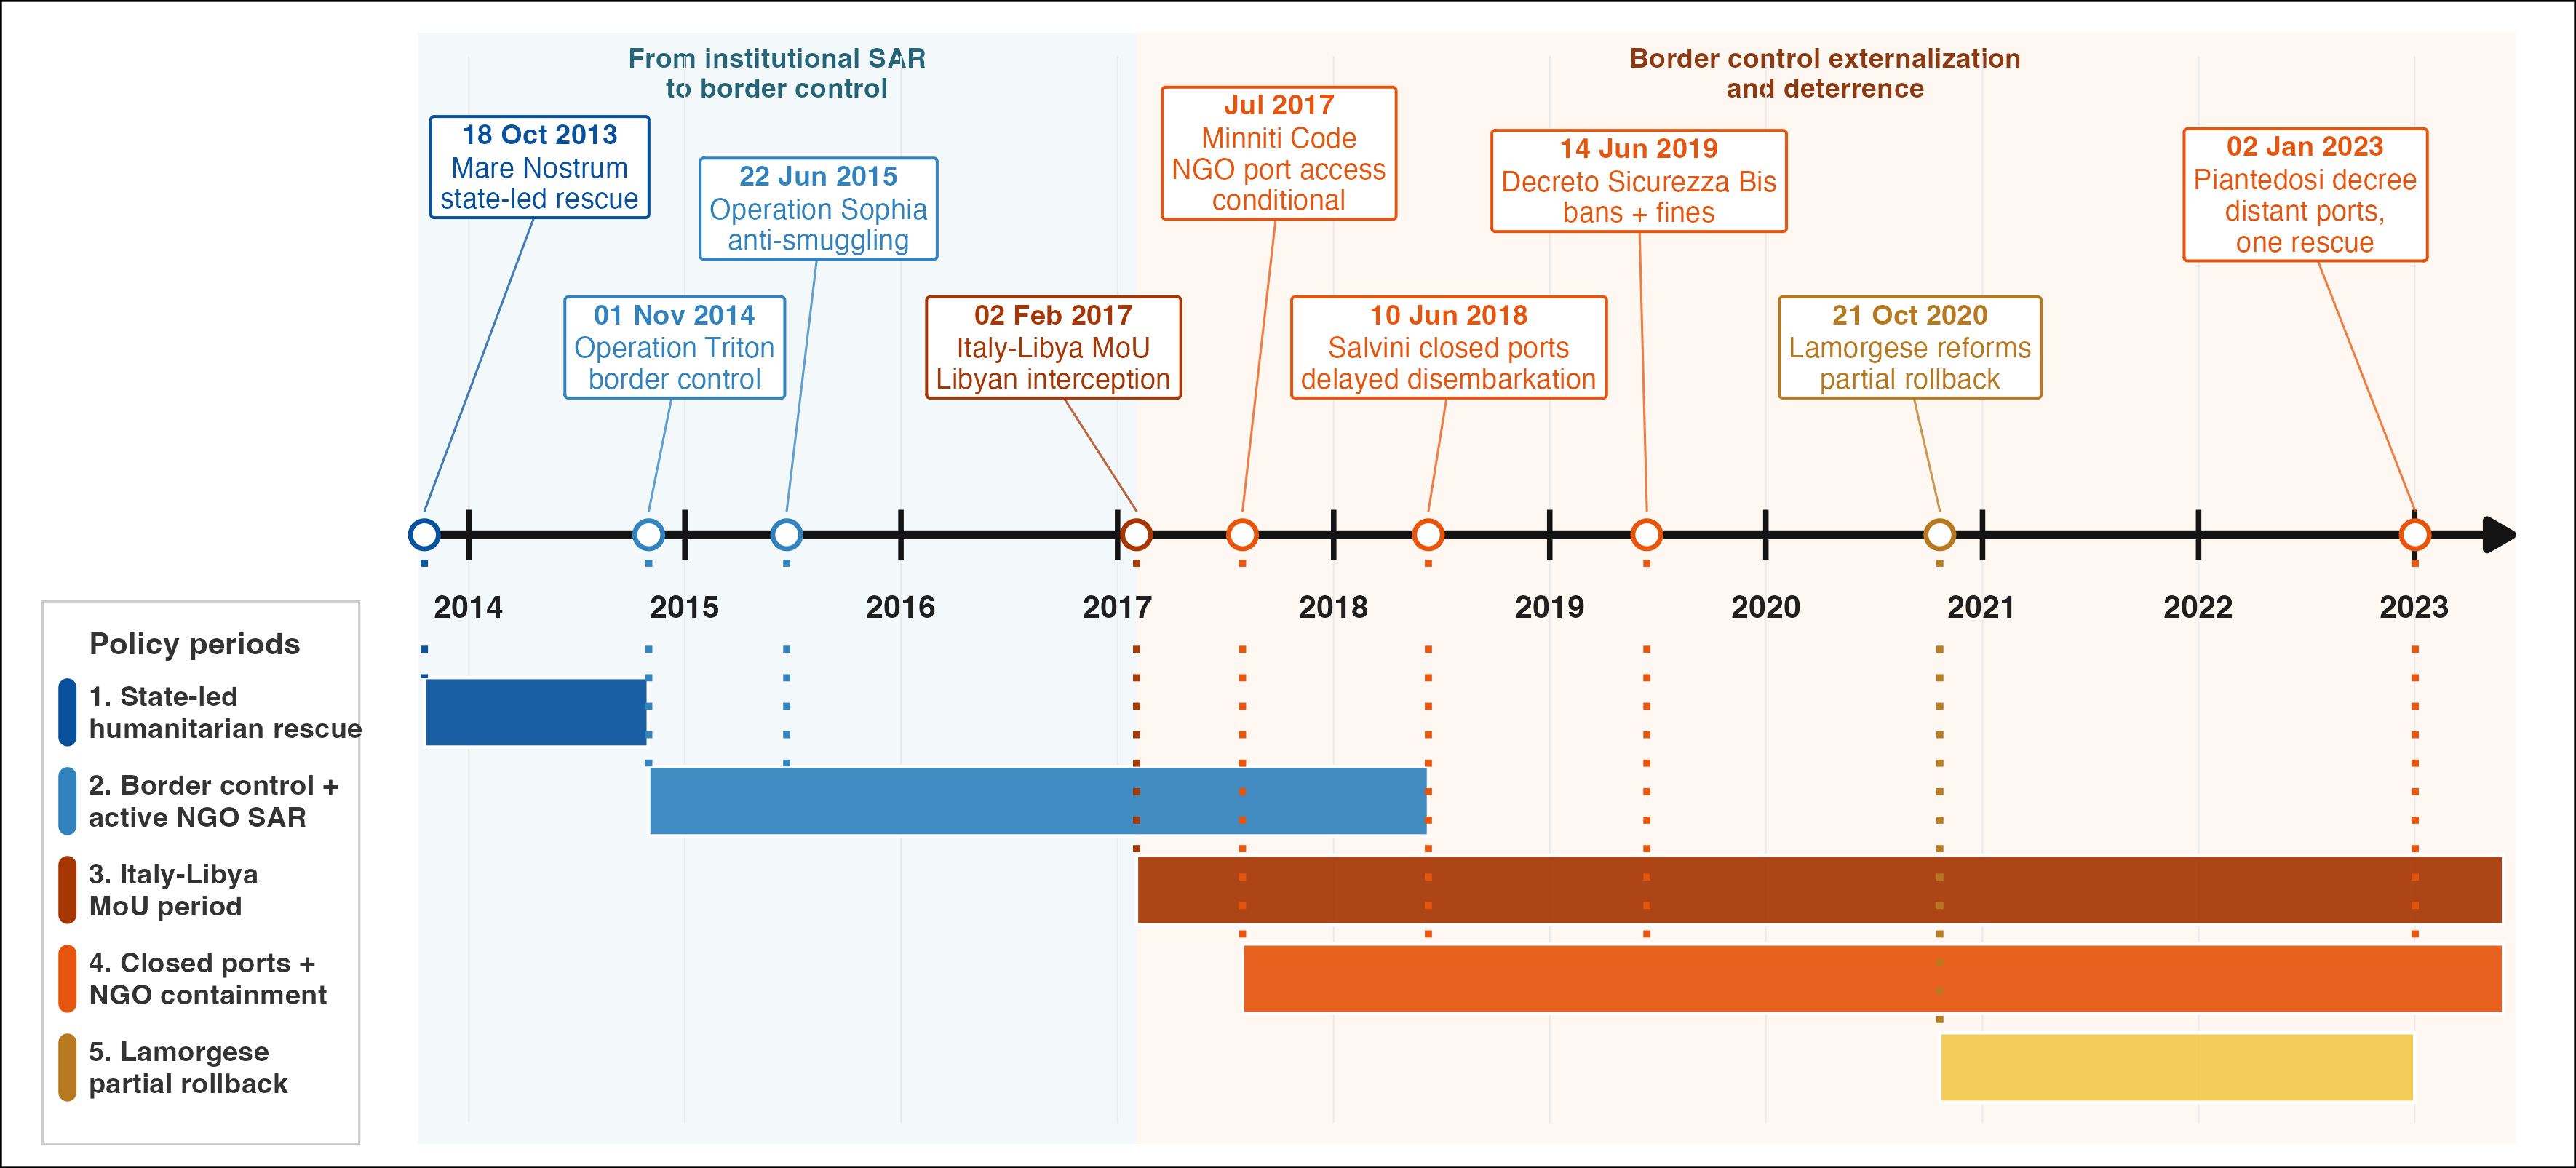
\includegraphics[width=\linewidth]{fig-policy-timeline.png}\end{whitecard}
  \figcap{Central Mediterranean rescue and border-control policy, 2013--2023.}
  \gp

  \figtitle{Fig 2 \textbar\ The corridor and SAR zones}
  \begin{whitecard}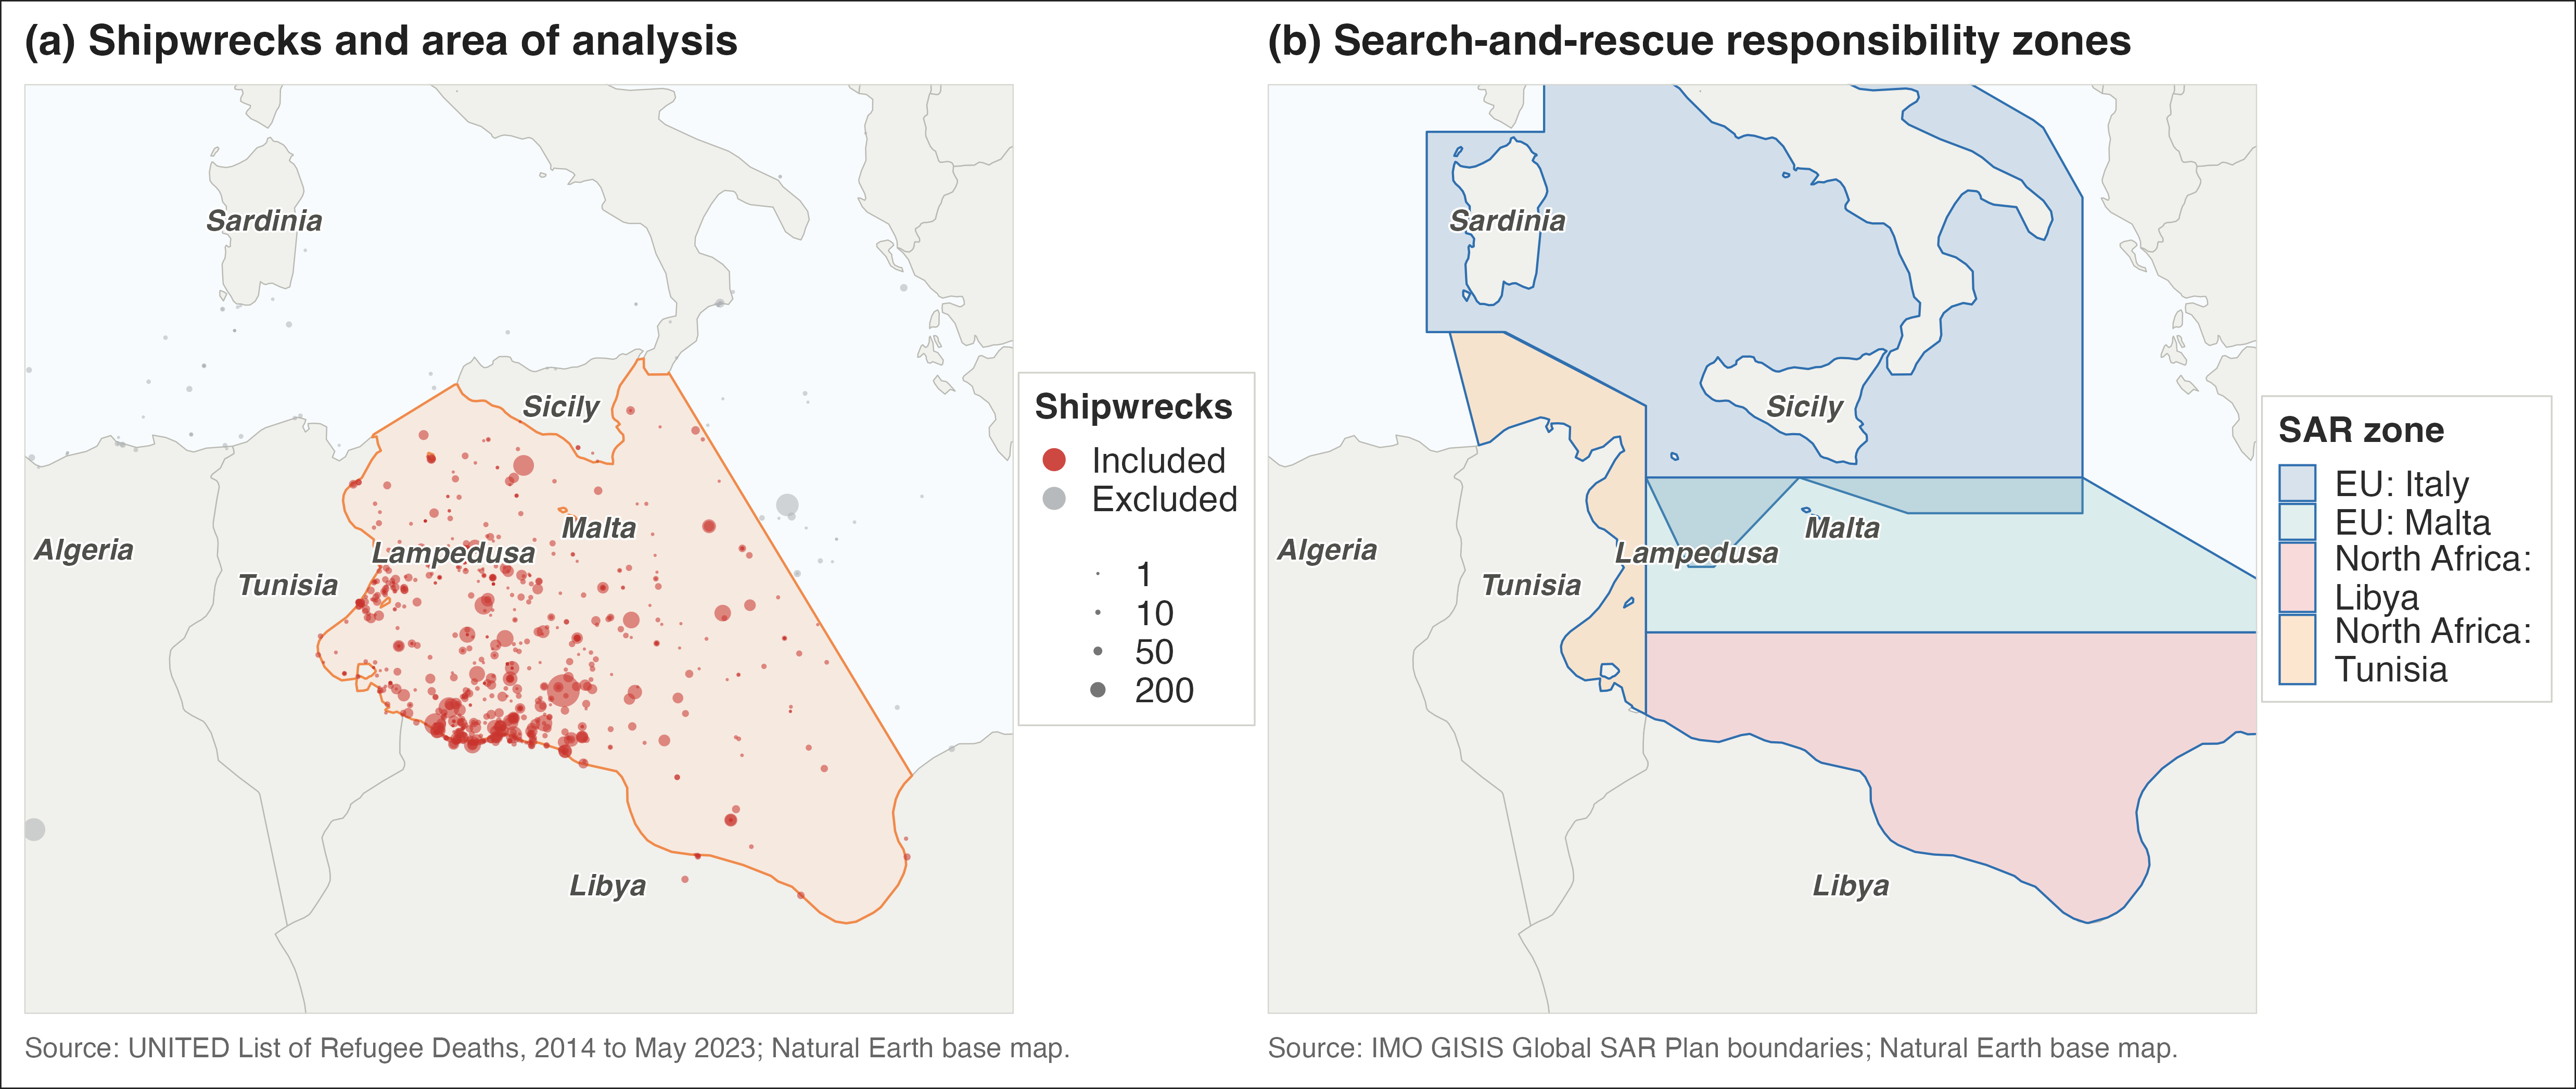
\includegraphics[width=\linewidth]{fig-sea-zones-united-sar-panel.png}\end{whitecard}
  \figcap{Area of analysis, UNITED deadly incidents, and the Italian, Maltese, Libyan and
   Tunisian search-and-rescue responsibility zones.}
\end{minipage}\hfill
% ===== RIGHT COLUMN =========================================================
\begin{minipage}[t]{\col}
  \vspace{0pt}
  \begin{panel}{\sechead{4}{Identification: exogenous sea-state variation}}
    Day-to-day sea state is \textbf{plausibly exogenous} to migration policy: the same
    rough weather recurs before and after 2017, whoever governs rescue. Conditional on
    month--year fixed effects, we ask how the slope from lagged SWH to recorded deaths
    \textbf{shifts} across the MoU.
    \textbf{Main limits}: no untreated comparison route and incomplete records; observed
    boat composition is checked, but unobserved timing, route choice, boat quality and
    crowding still limit attribution to SAR alone.
  \end{panel}
  \gp

  \begin{tcolorbox}[colback=darkcell, colframe=amber, boxrule=1.4pt, arc=3mm,
                    left=6mm, right=6mm, top=4.5mm, bottom=5mm]
    {\centering
     {\bfseries\color{white}\fontsize{23pt}{27pt}\selectfont The model}\\[3mm]
     {\fontsize{23pt}{28pt}\selectfont\color{white}
      $\mathbb{E}[D_t]=\exp\!\big(\alpha_{m(t)}+\beta_1 s_t+\textcolor{amber}{\beta_3}\, s_t\!\times\!\mathrm{Post}_t\big)$}\\[3mm]\par}
    {\fontsize{18pt}{24pt}\selectfont\color{muted}\justifying\setlength{\parindent}{0pt}
     A negative-binomial and Poisson \textbf{count model} with month--year fixed effects;
     $s_t$ is the lagged 5-day mean wave height and $\mathrm{Post}_t=1$ after the MoU. The
     estimand is \textcolor{amberlt}{$\beta_3$}: how much the wave-height-to-deaths slope
     shifts after 2017.\par}
  \end{tcolorbox}
  \gp

  \figtitle{Fig 3 \textbar\ Crossings and interceptions}
  \begin{whitecard}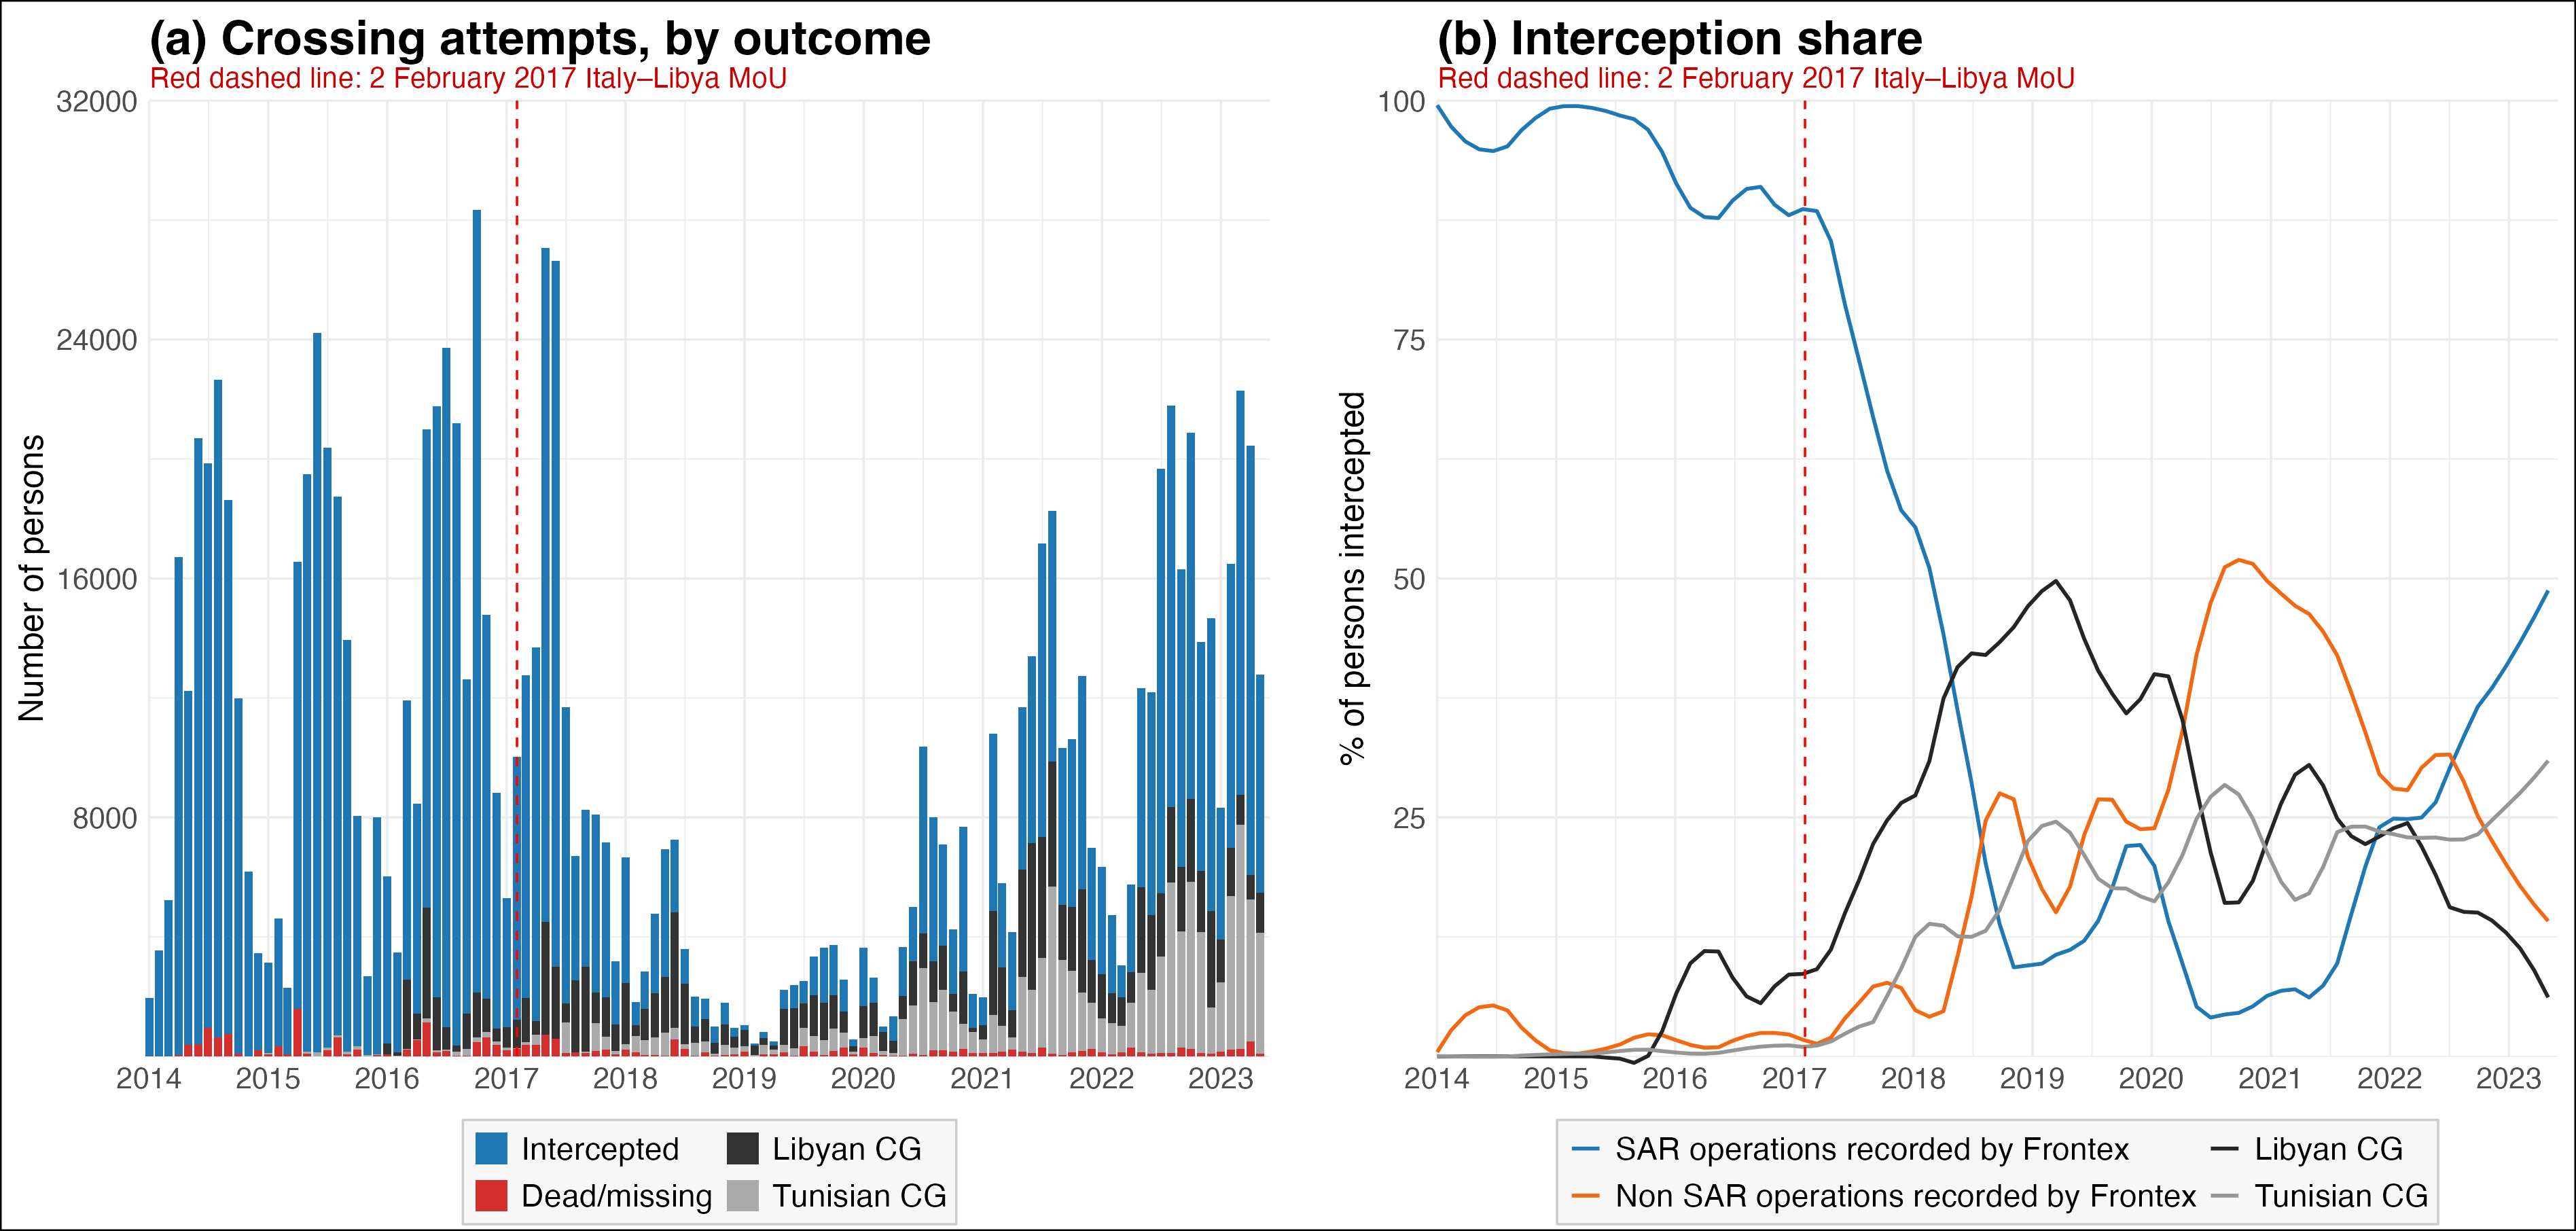
\includegraphics[width=\linewidth]{fig-crossings-ad.png}\end{whitecard}
  \figcap{Persons attempting the crossing by outcome, and the share intercepted by
   operation type, 2014--2023.}
  \gp

  \begin{panel}{\sechead{5}{Result: rough seas became riskier}}
    In the primary UNITED negative-binomial model, rougher seas predicted about
    \textbf{\color{white}94\% fewer} recorded deaths before the MoU. The post-MoU
    interaction adds $+3.63$, so the implied post-MoU slope is $+0.80$. With the log link,
    $\exp(0.80)=2.23$: expected deaths are \textbf{\color{white}2.23 times as high} per
    additional metre of lagged SWH.
    \vspace{2.2mm}
    \begin{tcolorbox}[colback=darkcell, colframe=rule, boxrule=0.8pt, arc=2mm,
                      left=5.5mm, right=5.5mm, top=3.4mm, bottom=3.4mm]
      {\fontsize{20pt}{27pt}\selectfont\color{ink}
       \setlength{\extrarowheight}{1mm}\arrayrulecolor{rule}
       \begin{tabularx}{\linewidth}{@{}>{\raggedright\arraybackslash}p{0.36\linewidth} l >{\raggedright\arraybackslash}X@{}}
         Parameter & Estimate & Interpretation\\[1mm]
         \hline
         Pre-MoU slope $\beta_1$            & $-2.83^{***}$                             & rough seas lower deaths\\[1mm]
         Post-MoU shift $\beta_3$           & {\color{amber}$\boldsymbol{+3.63^{***}}$} & adds to pre-MoU SWH effect\\[1mm]
         Implied post-MoU $\beta_1+\beta_3$ & {\color{amberlt}$\boldsymbol{+0.80^{*}}$} & rough seas increase deaths by $2.23\times$ per +1m SWH\\
       \end{tabularx}}\par\vspace{2.2mm}
      {\fontsize{16.5pt}{20.5pt}\selectfont\color{muted}\justifying\setlength{\parindent}{0pt}
       UNITED NegBin, month--year FE, Newey--West SEs (lag 14). Estimates are log slopes.}
    \end{tcolorbox}
    \vspace{2.2mm}
    The shift holds in both registries and both count models, and survives controls for
    crossing volume, boat composition and Libyan conflict.
  \end{panel}
  \gp

\begin{conclbox}{\sechead{6}{Contribution of the research}}
This thesis estimates how the \textbf{per-crossing risk of death} on the
CMR changed after the 2017 MoU. It asks whether sea-state hazard mapped into a different 
mortality gradient under the post-MoU period. The point is not only
whether deterrence reduced departures or arrivals, but whether crossings
became more dangerous.

  \vspace{2mm}

The evidence is consistent with SAR acting as a
\textbf{safety buffer}: after the MoU, rough seas became more strongly
associated with recorded deaths, \emph{even as crossings declined}.
The thesis proposes a new way to measure the human cost of this policy approach.
\end{conclbox}

\end{minipage}

% ---- Footer -----------------------------------------------------------------
\vfill
{\color{rule}\rule{\textwidth}{1.2pt}}
\vspace{3mm}
\noindent\begin{minipage}{\textwidth}
  \fontsize{18.5pt}{23pt}\selectfont\color{muted}
  \centering
  {\color{ink}\textbf{Giorgio Coppola}}\quad Hertie School, Class of 2026 \qquad
  {\color{amber}\faEnvelope}\ \,\href{mailto:coppola.giorgio99@gmail.com}{coppola.giorgio99@gmail.com} \qquad
  {\color{amber}\faLinkedin}\ \,\href{http://linkedin.com/in/giorgio-coppola}{linkedin.com/in/giorgio-coppola} \qquad
  {\color{amber}\faGithub}\ \,\href{http://github.com/giocopp/thesis-cmr-mortality}{github.com/giocopp/thesis-cmr-mortality}
\end{minipage}

\end{document}
